\documentclass[12pt]{article}
%\usepackage[margin=1in]{geometry}% Change the margins here if you wish.
%\setlength{\parindent}{0pt} % This is the set the indent length for new paragraphs, change if you want.
%\setlength{\parskip}{5pt} % This sets the distance between paragraphs, which will be used anytime you have a blank line in your LaTeX code.
%\pagenumbering{gobble}% This means the page will not be numbered. You can comment it out if you like page numbers.

%------------------------------------

\usepackage{color}
\usepackage[utf8]{inputenc}
\usepackage{hyperref}
\usepackage{listings}% http://ctan.org/pkg/listings


\usepackage{cprotect}
\usepackage{mathtools}

\usepackage{comment}
\linespread{1.6}

% These packages allow the most of the common "mathly things"
\usepackage{amsmath,amsthm,amssymb}

% This package allows you to add images.
\usepackage{graphicx}
\usepackage{float}

\usepackage{listings}

\newcommand{\grn}{\textcolor{green}}
\newcommand{\red}{\textcolor{red}}
\newcommand\todo[1]{\red{\Large \text{TODO: #1}}}
\newcommand{\defeq}{\vcentcolon=}
\newcommand{\eqdef}{=\vcentcolon}
\newcommand\Item[1][]{%
  \ifx\relax#1\relax  \item \else \item[#1] \fi
  \abovedisplayskip=0pt\abovedisplayshortskip=0pt~\vspace*{-\baselineskip}}
\newcommand\eb[1]{[[\texttt{#1}]]}
% Should you need any additional packages, you can load them here. If you've looked up something (like on DeTeXify), it should specify if you need a special package.  Just copy and paste what is below, and put the package name in the { }.  
\usepackage{wasysym} %this lets me make smiley faces :-)

\title{CML - Uma Linguagem para {\it Machine Learning} \\ \Large Relatório 2 - Trabalho de Conceitos de Linguagem de Programação}

\author{Caio Lopes, Leonardo Blanger, Marcelo Silvarolla}

\date{16 de maio de 2018}

\begin{document}
\lstset{
  basicstyle=\ttfamily,
  columns=fullflexible,
  keepspaces=true,
  mathescape
}

\maketitle
\tableofcontents
\newpage
\section{Sintaxe Concreta}
Usamos a seguinte notação para nossas regras EBNF:
\begin{center}
\begin{tabular}{c c}
definição  : \\
concatenação  (espaço) \\
união  $\vert$  \\
agrupamento  ($\ldots$) \\
{\it string} terminal  \verb!"!$\ldots$\verb!"! \\
{\it string} terminal  '$\ldots$' \\
*  zero ou mais \\
+  um ou mais \\
/* $\ldots$ */  comentário \\
terminação  ;
\end{tabular}
\end{center}

O alfabeto, isto é, o conjunto de símbolos terminais da nossa linguagem, será o conjunto de caracteres ASCII, conforme a tabela:
\begin{center}
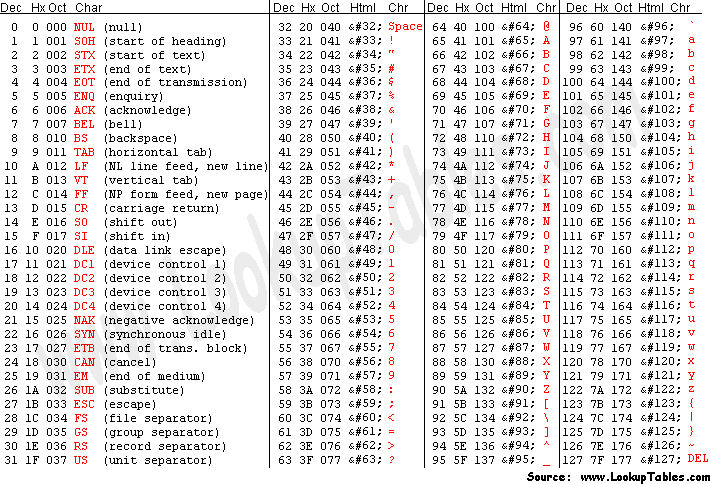
\includegraphics[width=\linewidth,height=\textheight,keepaspectratio]{asciitable.png}
\end{center}
\subsection{Palavras Reservadas}
{\tt char else real bool string dataset model if int return void while skip \\ || < <= > >= == != ; \{ \} , = ( ) [ ] ! - + * /}
\subsection{Regras Léxicas}
Os espaços são ignorados na análise léxica.
Denotaremos os {\it tokens} por seus nomes em LETRAS MAIÚSCULAS, para os diferenciar dos demais símbolos não-terminais.

\todo{Ajeitar as aspas simples}

\begin{verbatim}
D : "0" | "1" | "2" | "3" | "4" | "5" | "6" | "7" | "8" | "9";
L : "A" | "B" | "C" | "D" | "E" | "F" | "G"
       | "H" | "I" | "J" | "K" | "L" | "M" | "N"
       | "O" | "P" | "Q" | "R" | "S" | "T" | "U"
       | "V" | "W" | "X" | "Y" | "Z" | "a" | "b"
       | "c" | "d" | "e" | "f" | "g" | "h" | "i"
       | "j" | "k" | "l" | "m" | "n" | "o" | "p"
       | "q" | "r" | "s" | "t" | "u" | "v" | "w"
       | "x" | "y" | "z" | "_";
A : L | D;
ES : "\" ("'" | '"' | "\" | "n" | "t");
CHAR : "char";
ELSE : "else";
REAL : "real";
BOOL : "bool";
STRING : "string";
DATASET : "dataset";
MODEL : "model";
IF : "if";
INT : "int";
RETURN : "return";
VOID : "void";
WHILE : "while";
SKIP : "skip";
IDENTIFIER : L (A)*;
INT_LITERAL : (D)+;
REAL_LITERAL : (D)* "." (D)+ | (D)+ ".";
NONQUOTE_BACKSLASH_NEWLINE :
' ' | '!' | '"' | '#' | '$' | '%' | '' | "'" | '(' | ')' | 
'*' | '+' | ',' | '-' | '.' | '/' | '0' | '1' | '2' | '3' | 
'4' | '5' | '6' | '7' | '8' | '9' | ':' | ';' | '<' | '=' | 
'>' | '?' | '@' | 'A' | 'B' | 'C' | 'D' | 'E' | 'F' | 'G' | 
'H' | 'I' | 'J' | 'K' | 'L' | 'M' | 'N' | 'O' | 'P' | 'Q' | 
'R' | 'S' | 'T' | 'U' | 'V' | 'W' | 'X' | 'Y' | 'Z' | '[' | 
'\' | ']' | '^' | '_' | '`' | 'a' | 'b' | 'c' | 'd' | 'e' | 
'f' | 'g' | 'h' | 'i' | 'j' | 'k' | 'l' | 'm' | 'n' | 'o' | 
'p' | 'q' | 'r' | 's' | 't' | 'u' | 'v' | 'w' | 'x' | 'y' | 
'z' | '{' | '|' | '}' | '~';
CHAR_LITERAL : "'" (NONQUOTE_BACKSLASH_NEWLINE | '"' | ES)"'";
STRING_LITERAL : '"' (NONQUOTE_BACKSLASH_NEWLINE | "'" | ES)* '"';
AND_OP : "&&";
OR_OP : "||";
LE_OP : "<=";
GE_OP : ">=";
EQ_OP : "==";
NE_OP : "!=";
\end{verbatim}
\footnote{\texttt{D} de dígito, \texttt{L} de letra, \texttt{A} de alfanumérico (letra ou dígito), \texttt{ES} de {\it escape sequence}.  Note que incluímos o {\it underscore} como letra.

O não-terminal \texttt{NONQUOTE\_BACKSLASH\_NEWLINE} define o conjunto de todos os caracteres ASCII imprimíveis que não são uma aspa simples, aspa dupla, barra inversa ou quebra de linha.}

\subsection{Regras Sintáticas}
\subsubsection{Símbolos Terminais}
Os símbolos terminais na análise sintática são os {\it tokens} gerados na análise léxica acima.
\subsubsection{Expressões}
Os espaços são ignorados na análise léxica.
\begin{verbatim}
/* Expressões necessariamente "atômicas":
    Expressões que não causam ambiguidades quando dentro
    de uma expressão maior, mesmo quando a precedência
    das operações não é conhecida
    Estas expressões podem, portanto, ser pensadas
    como identificadores ou literais. */

primary_expression
    : IDENTIFIER
    | literal
    | '{' '}'
    | '{' expression_list '}'
    | '(' expression ')'
    | array_access
    | IDENTIFIER '(' ')'
    | IDENTIFIER '(' expression_list ')'
    ;

literal
    : INT_LITERAL
    | REAL_LITERAL
    | BOOL_LITERAL
    | CHAR_LITERAL
    | STRING_LITERAL
    ;

/* Expressões "não-atômicas" */
expression_list
    : expression
    | expression_list ',' expression
    ;

expression
    : logical_or_expression
    | IDENTIFIER '=' expression
    | array_access '=' expression
    ;

array_access
    : IDENTIFIER '[' expression ']'
    | array_access '[' expression ']'
    ;

logical_or_expression
    : logical_and_expression
    | logical_or_expression OR_OP logical_and_expression
    ;

logical_and_expression
    : relational_expression
    | logical_and_expression AND_OP relational_expression
    ;

relational_expression
    : additive_expression
    | additive_expression '<' additive_expression
    | additive_expression '>' additive_expression
    | additive_expression LE_OP additive_expression
    | additive_expression GE_OP additive_expression
    | additive_expression EQ_OP additive_expression
    | additive_expression NE_OP additive_expression
    ;

additive_expression
    : multiplicative_expression
    | additive_expression '+' multiplicative_expression
    | additive_expression '-' multiplicative_expression
    ;

multiplicative_expression
    : unary_minus_expression
    | multiplicative_expression '*' unary_minus_expression
    | multiplicative_expression '/' unary_minus_expression
    ;

unary_minus_expression
    : neg_expression
    | '-' neg_expression
    ;

neg_expression
    : primary_expression
    | '!' neg_expression
    ;
\end{verbatim}


\subsubsection{Comandos}
\begin{verbatim}
command
    : compound_command
    | expression_command
    | selection_command
    | iteration_command
    | jump_command
    | SKIP ';'
    ;

compound_command
    : '{' declaration_or_command_list '}'
    ;

declaration_or_command_list 
    : declaration_or_command
    | declaration_or_command_list declaration_or_command
    ;

declaration_or_command
    : declaration
    | command
    ;

expression_command
    : ';'
    | expression ';'
    ;

selection_command
    : IF '(' expression ')' compound_command ELSE compound_command
    | IF '(' expression ')' compound_command
    ;

iteration_command
    : WHILE '(' expression ')' command
    ;

jump_command
    : RETURN ';'
    | RETURN expression ';'
    ;
\end{verbatim}

\subsubsection{Declarações}
\begin{verbatim}
declaration
    : type_specifier IDENTIFIER ';'
    | type_specifier IDENTIFIER '=' expression ';'
    | type_specifier IDENTIFIER '(' ')' ';'
    | type_specifier IDENTIFIER '(' parameter_declaration_list ')' ';'
    ;

parameter_declaration_list
    : parameter_declaration
    | parameter_declaration_list ',' parameter_declaration
    ;

parameter_declaration
    : type_specifier IDENTIFIER
    ;

type_specifier
    : VOID
    | CHAR
    | INT
    | REAL
    | BOOL
    | STRING
    | DATASET
    | MODEL
    | type_specifier '[' ']'
    ;
\end{verbatim}

\subsubsection{Definições}
\begin{verbatim}
function_definition
    : type_specifier IDENTIFIER '(' ')' compound_command
    | type_specifier IDENTIFIER '(' 
    parameter_declaration_list ')' compound_command
    ;
\end{verbatim}

\subsubsection{Programa}
\begin{verbatim}
program
    : declaration_or_function_definition
    | program declaration_or_function_definition
    ;

declaration_or_function_definition
    : function_definition
    | declaration
    ;

\end{verbatim}
\subsection{Exemplo}
\todo{EXEMPLO}
\section{Semântica}

\subsection{Domínios Sintáticos}

\begin{itemize}
\item {\tt Identifier $\defeq$} conjunto de todas as sequências finitas de terminais deriváveis a partir do não-terminal {\tt IDENTIFIER} acima.

\item {\tt Literal $\defeq$} conjunto de todas as sequências finitas de terminais deriváveis a partir do não-terminal {\tt literal} acima.

\item {\tt ArrayAccess $defeq$} conjunto de todas as sequências finitas de terminais deriváveis a partir do não-terminal {\tt arr\_access} acima.

\item {\tt Expression $\defeq$} conjunto de todas sequências finitas de terminais deriváveis a partir do não-terminal {\tt exp} abaixo.

\item {\tt Command $\defeq$} conjunto de todas as sequências finitas de terminais deriváveis a partir do não-terminal {\tt cmd} abaixo.

\item {\tt Declaration $\defeq$} conjunto de todas as sequências finitas de terminais deriváveis a partir do não-terminal {\tt dec} abaixo.

\item {\tt FunctionDefinition $\defeq$} conjunto de todas as sequências finitas de terminais deriváveis a partir do não-terminal {\tt function\_def} abaixo.

\item {\tt Program $\defeq$} conjunto de todas as sequências finitas de terminais deriváveis a partir do não-terminal {\tt prog} abaixo.

\end{itemize}



\subsection{Sintaxe Abstrata}
A sintaxe em EBNF acima contém detalhes irrelevantes para a semântica, especificando formalmente a associatividade e precedência dos operadores. Aqui, apresentamos uma sintaxe simplificada, a sintaxe abstrata, que, apesar de ambígua, é suficiente para a definição da semântica. Estamos essencialmente seguindo o capítulo $9$ do livro de Kenneth Slonneger e Barry L. Kurtz "Formal Syntax and Semantics of Programming Languages"\footnote{Disponível em \url{http://www.divms.uiowa.edu/~slonnegr/plf/Book/Chapter9.pdf}}.
Observe que \verb!IDENTIFIER! e \verb!literal! estão definidos na sintaxe concreta acima.
\subsubsection{Expressões}

\begin{verbatim}
id : IDENTIFIER;
lit : literal;
exp_list : exp | exp_list "," exp;
arr_access : id | arr_access "[" exp "]";
exp : id | lit | "{" "}" | "{ exp_list "}" |
     exp "||" exp | arr_access "=" exp | exp "&&" exp |
     exp "==" exp | exp "!=" exp | exp "<" exp | exp "<=" exp |
     exp ">" exp | exp ">=" exp | "-" exp | exp "+" exp |
     exp "-" exp | exp "*" exp | exp "/" exp |
     "(" exp ")" | exp "[" exp "]" | id "(" ")" |
     id "(" exp_list ")" | "!" exp;
\end{verbatim}

\subsubsection{Comandos}
\begin{verbatim}
cmd : comp_cmd | exp_cmd | 
       sel_cmd | iter_cmd |
       jump_cmd | SKIP ";";
comp_cmd : "{" (dec | cmd)+ "}";
exp_cmd : exp ";";
sel_cmd : IF "(" exp ")" comp_cmd ELSE comp_cmd |
                 IF "(" exp ")" comp_cmd;
iter_cmd : WHILE "(" exp ")" cmd;
jump_cmd : RETURN ";" | RETURN exp ";";
\end{verbatim}

\subsubsection{Declarações}
Note que \verb!type_specifier! está definido na sintaxe concreta acima.
\begin{verbatim}
type_spec : type_specifier;
dec : type_spec id ";" | 
       type_spec id "=" exp ";" |
       type_spec id "(" ")" ";" |
       type_spec id "(" param_dec_list ")" ";";
param_dec : type_spec id;
param_dec_list : param_dec | param_dec_list "," param_dec;
\end{verbatim}

\subsubsection{Definições}

\begin{verbatim}
fun_def : type_spec id "(" ")" comp_cmd |
         type_spec id "(" param_dec_list ")" comp_cmd;
\end{verbatim}

\subsubsection{Programa}

\begin{verbatim}
prog : dec_or_fun_def | prog dec_or_fun_def;
dec_or_fun_def : fun_def | dec;
\end{verbatim}

\subsection{Domínios Semânticos}

Denotamos por $X \rightarrow Y$ o conjunto de funções parciais de $X$ em $Y$. Escrevemos $f:X \rightarrow Y$ para dizer que $f$ é função parcial de $X$ em $Y$. Ademais, se $n\in\mathbb{N}$, $X^n \defeq X \times \ldots (n \text{ vezes }) \ldots \times X \defeq \{f \mid f \text{ é função total do conjunto } \{0, 1, \ldots, n-1\}\text{ em } X\}$ é o conjunto de tuplas (isto é, vetores) de $n$ elementos de $X$. Por exemplo, $\mathbb{R}\to\mathbb{R}$ é o conjunto de todas as funções da reta na reta, enquanto $\mathbb{R}^n$ é o espaço euclidiano $n$-dimensional.

\begin{itemize}
\item $Int \defeq \{\ldots, -2, -1, 0, 1, 2, \ldots\} = \mathbb{Z}$

\item $Real \defeq  \mathbb{R}$
\item $Bool \defeq \{true, false\}$
\item $Char \defeq \{0, \ldots, 127\}$, onde os números de 0 a 127 são interpretados conforme o padrão ASCII, e.g., 43 representa `$+$', 49 representa `1', etc. Para mais detalhes, ver tabela no início do relatório.

Definimos, para cada conjunto $X$, o conjunto $X[]$ dos vetores de elementos de $X$ pondo $X[] \defeq \bigcup_{n = 0}^{+\infty} X^n$

$rotulo(X)$ denota o conjunto $\{rotulo(x): x\in X\}$ de elementos de $X$ rotulados pela palavra {\it rotulo}. Por exemplo, $$int(Int) = \{\ldots, int(-2), int(-1), int(0), int(1), int(2), \ldots\}.$$ Isto serve para que possamos tomar a união, por exemplo, $int(Int) \cup char(Char)$, que é 
$$\{\ldots, int(-2), int(-1), int(0),  int(1), int(2), \ldots, char(0), char(1), \ldots, char(127)\},$$
e saber de que conjunto cada elemento provém. Se simplesmente tomássemos a união sem rótulos, $Int \cup Char = Int$, não saberíamos, por exemplo, se $5\in Int \cup Char$ provém do conjunto $Int$ ou do conjunto $Char$, isto é, não saberíamos o tipo do valor $5$.

\item $String = Char[]$

Observe que $String$ é simplesmente o conjunto dos vetores de $Char$'s. Usaremos os rótulos $string$ e $array$ para distingui-los.

\item $Dataset = \{0, \ldots, n\} \times \{1, \ldots, m\} \rightarrow int(Int) \cup real(Real) \cup string(String)$

\item $Model = Dataset \rightarrow Dataset$

\Item \begin{align*} 
Array = & int(Int)[] \cup real(Real)[] \cup bool(Bool)[]\cup char(Char)[] \\ 
&\cup string(String)[] \cup dataset(Dataset)[] \cup model(Model)) \\
&\cup int(Int)[][] \cup real(Real)[][] \cup bool(Bool)[][]\cup char(Char)[][] \\
&\cup string(String)[][] \cup dataset(Dataset)[][] \cup model(Model)[][] \\
&\cup int(Int)[][][] \cup \ldots\text{\footnotemark}
\end{align*}
\footnotetext{Note que $int[]$ é meramente um rótulo, um nome, enquanto que $Int[]$ é o conjunto de vetores de $Int$'s.}
\item $Input \defeq \bigcup_{n = 0}^{+\infty} Dataset^n$
\item $Output \defeq \bigcup_{n = 0}^{+\infty} Dataset^n$

\item $Function = \bigcup_{n = 0}^{+\infty} (Location^n \rightarrow Store \times Input \times Output)$

\item $StorableValue \defeq int(Int) \cup real(Real) \cup bool(Bool) \cup char(Char) \cup string(String) \cup dataset(Dataset) \cup model(Model) \cup array(Array)$
\item $ExpressibleValue \defeq StorableValue$

\item $DenotableValue \defeq var(Location) \cup fun(Function)$
\item $Location \defeq \mathbb{N} \defeq \{0, 1, 2, \ldots\}$
\item $Environment \defeq {\tt Identifier} \to DenotableValue \cup \{unbound\}$\footnote{O valor $unbound$ indica que o identificador não foi associado a uma posição de memória ou função, isto é, não foi declarado.}
\item $Store \defeq Location\to StorableValue \cup \{unused\} \cup \{undefined\}$\footnote{O valor $unused$ indica que a localização não está sendo utilizada por nenhuma variável. Já o valor $undefined$ indica que a localização está sendo utilizada por uma variável que não foi inicializada.}

\item $\Sigma \defeq State \defeq Environment \times Store \times Input \times Output$


\end{itemize}

Obs.: acrescentamos o valor especial $error$ em todos os domínios, para indicar erro no programa e supomos que erros são propagados pelas funções semânticas.

\subsection{Funções Semânticas}
Todas as funções abaixo de fato podem precisar do estado completo $\Sigma$ do programa, incluindo $Environment$, $Store$, $Input$ e $Output$. Porém:
\begin{itemize}
\item Uma ${\tt Expression}$ não precisa devolver o $Environment$, já que não o modifica. Basta, então, devolver $Store$, $Input$,  $Output$ e, obviamente, um $ExpressibleValue$.
\item Idem para um {\tt Command}
\item Uma {\tt Declaration} pode alterar o estado completo: $Environment$, $Store$, $Input$ e $Output$.
\item Uma {\tt FunctionDefinition} pode alterar apenas o $Environment$, ligando um $Identifier$ de função com a $Function$ correspondente.
\item Um {\tt Program} pode alterar o estado completo: $Environment$, $Store$, $Input$ e $Output$.
\end{itemize}
\begin{align*}
E   &:{\tt Expression} \rightarrow (\Sigma \rightarrow Store \times Input \times Output \times ExpressibleValue) \\
C   &:{\tt Command} \rightarrow (\Sigma \rightarrow Store \times Input \times Output) \\
Dec &:{\tt Declaration} \rightarrow (\Sigma \rightarrow \Sigma) \\
Def &:{\tt FunctionDefinition} \rightarrow (\Sigma \rightarrow Environment) \\
P   &:{\tt Program} \rightarrow (\Sigma \rightarrow \Sigma)
\end{align*}
Além disso, teremos as seguintes funções auxiliares (algumas de $0$ argumentos, como $emptyEnv$):

\todo{especificar funções predefinidas de CML}
\begin{align*}
&value:Literal\to int(Int)\cup real(Real)\cup bool(Bool)\cup  char(Char)\cup string(String)\footnotemark\\
&emptyEnv:Environment \\
&extendEnv:Environment\times Identifier\times DenotableValue\to Environment \\
&applyEnv:Environment\times Identifier\to DenotableValue\cup \{unbound\} \\
&emptySto:Store \\
&updateSto:Store\times Location \times \big(StorableValue \cup \{undefined, unused\}\big) \to Store \\
&applySto:Store\times Location \to StorableValue\cup \{undefined, unused\} \\
&allocate:Store\to Store\times Location \\
&deallocate:Store\times Location \to Store \\
\end{align*}\footnotetext{Por exemplo:
\begin{align*}
&value(\text{{\tt 101}}) = int(101) \\
&value(\text{{\tt true}}) = bool(true) \\
&value(\text{{\tt 5.2}}) = real(5,2) \\
&value(\text{{\tt "Maria"}}) = string(``Maria") \\
\end{align*}}
\subsection{Equações Semânticas}
Quando mais de uma equação é fornecida para uma mesma função semântica, supõe-se que a primeira que servir para o argumento é executada. As demais são ignoradas. Há aqui, portanto, uma analogia com linguagens funcionais como Haskell e SML, que possuem {\it pattern matching}.
\subsubsection{Funções auxiliares}
\todo{definir value e funções predefinidas de CML} 
\begin{align*}
&value\\
&emptyEnv\ I = unbound \\
&extendEnv(env, I, dval) \;I_1 = \big(\textbf{if } I_1 = I \textbf{ then } dval \textbf{ else } env(I_1)\big) \\
&applyEnv(env, I) = env(I) \\
&emptyStore\ loc = unused \\
&updateSto(sto,loc,val) \;loc_1 = \big( \textbf{if $loc_1 = loc$ then $val$ else $sto(loc_1)$}\big) \\
&applySto(sto, loc) = sto(loc)\\
&allocate \;sto = (updateSto(sto, loc, undefined), loc) \\
&\hspace{6ex} \textbf{where } loc = minimum \{k \mid sto(k) = unused\} \\
&deallocate(sto,loc) = updateSto(sto,loc,unused)
\end{align*} 
\subsubsection{Programa}

\begin{align*}
&P\;\eb{dec} \;\sigma = Dec\;\eb{dec} \;\sigma \\
&P\;\eb{{\bf int main()} comp\_cmd} \;(env,sto,in,out) =
(env_2, sto_2, in_2, out_2) \\
	&\hspace{6ex}\textbf{where } env_1 = Def\;\eb{{\bf int main()} comp\_cmd} \;(env,sto,in,out) \\
	&\hspace{6ex}\textbf{and } (env_2,sto_2,in_2,out_2) = C\;[[comp\_cmd]] \;(env_1,sto,in,out) \\
&P\;\eb{type\_spec id(param\_dec\_list) comp\_cmd} \;(env,sto,in,out) = \\
&\hspace{6ex}(env_1, sto, in, out) \\
	&\hspace{6ex}\textbf{where } env_1 = Def\;\eb{type\_spec id(param\_dec\_list) comp\_cmd} \;(env,sto,in,out)\\
&P\;\eb{type\_spec id() comp\_cmd} \;(env,sto,in,out) = \\
&\hspace{6ex}(env_1, sto, in, out) \\
	&\hspace{6ex}\textbf{where } env_1 = Def\;\eb{type\_spec id() comp\_cmd} \;(env,sto,in,out)\\
&P\;\eb{prog dec\_or\_fun\_def} \;\sigma = P\;\eb{dec\_or\_fun\_def} (P\;\eb{prog} \;\sigma)
\end{align*}

\subsubsection{Expressões}

{\large \color{red} Falta a atribuição, as expressões que envolvem acessar posições de vetor, as chamadas de funções, e as expressões que envolvem arrays literais.}


\begin{align*}
&E\;\eb{id} \;(env, sto, in, out) = \text{ \bf if } val = undefined \text{ \bf then } error \text{ \bf else } (sto,in,out,val)  \\ 
&\hspace{6ex} \textbf{ where } val = applySto(sto, loc) \\
&\hspace{6ex} \textbf{ where } loc = applyEnv(env, \texttt{id}) \\
&E[[{\tt lit}]] (env,sto,in,out) = (sto,in,out,value(\texttt{lit})) \\
\end{align*}

\begin{align*}
&E[[{\tt \{\}}]] \;(env,sto,in,out) = (sto,in,out,array(\emptyset)) \\
&E[[{\tt \{exp\}}]] \;(env,sto,in,out) = (sto_1, in_1, out_1, array(val)) \\
&\hspace{6ex}\textbf{ where } (sto_1, in_1, out_1, val) = E[[{\tt exp}]] (env,sto,in,out) \\
&E[[{\tt exp\_list, exp}]] \;(env,sto,in,out) = (sto_2, in_2, out_2, array(extendArray(arr, val))) \\
&\hspace{6ex}\textbf{ where } (sto_1, in_1, out_1, arr) = E[[{\tt\{ exp\_list\}}]]\ (env, sto, in, out) \\
&\hspace{6ex}\textbf{ where } (sto_2, in_2, out_2, val) = E[[{\tt exp}]]\ (env, sto_1, in_1, out_1) \\
\end{align*}

\begin{align*}
E[[{\tt e_1 + e_2}]] \sigma = int(m + n) \textbf{ where } int(m) = E[[{\tt e_1}]] \sigma \textbf{ and } int(n) = E[[{\tt e_2}]] \sigma \\
                            = real(m + n) \textbf{ where } int(m) = E[[{\tt e_1}]] \sigma \textbf{ and } real(n) = E[[{\tt e_2}]] \sigma \\
                   = real(m + n) \textbf{ where } real(m) = E[[{\tt e_1}]] \sigma \textbf{ and } int(n) = E[[{\tt e_2}]] \sigma \\
                   = real(m + n) \textbf{ where } real(m) = E[[{\tt e_1}]] \sigma \textbf{ and } real(n) = E[[{\tt e_2}]] \sigma \\
\end{align*}

\begin{align*}
E[[{\tt e_1 - e_2}]] \sigma = int(m - n) \textbf{ where } int(m) = E[[{\tt e_1}]] \sigma \textbf{ and } int(n) = E[[{\tt e_2}]] \sigma \\
                            = real(m - n) \textbf{ where } int(m) = E[[{\tt e_1}]] \sigma \textbf{ and } real(n) = E[[{\tt e_2}]] \sigma \\
                   = real(m - n) \textbf{ where } real(m) = E[[{\tt e_1}]] \sigma \textbf{ and } int(n) = E[[{\tt e_2}]] \sigma \\
                   = real(m - n) \textbf{ where } real(m) = E[[{\tt e_1}]] \sigma \textbf{ and } real(n) = E[[{\tt e_2}]] \sigma \\
\end{align*}

\begin{align*}
E[[{\tt e_1 * e_2}]] \sigma = int(m \times n) \textbf{ where } int(m) = E[[{\tt e_1}]] \sigma \textbf{ and } int(n) = E[[{\tt e_2}]] \sigma \\
                            = real(m \times n) \textbf{ where } int(m) = E[[{\tt e_1}]] \sigma \textbf{ and } real(n) = E[[{\tt e_2}]] \sigma \\
                   = real(m \times n) \textbf{ where } real(m) = E[[{\tt e_1}]] \sigma \textbf{ and } int(n) = E[[{\tt e_2}]] \sigma \\
                   = real(m \times n) \textbf{ where } real(m) = E[[{\tt e_1}]] \sigma \textbf{ and } real(n) = E[[{\tt e_2}]] \sigma \\
\end{align*}

\begin{align*}
E[[{\tt e_1 / e_2}]] \sigma = \textbf{ if } n = 0 \textbf{ then } error \textbf{ else } int(m \div n) \\
\textbf{\hspace{5em}where } int(m) = E[[{\tt e_1}]] \textbf{ and } int(n) = E[[{\tt e_2}]] \sigma \\
                            = \textbf{ if } n = 0 \textbf{ then } error \textbf{ else } real(m \div n) \\
\textbf{\hspace{5em}where } real(m) = E[[{\tt e_1}]] \textbf{ and } int(n) = E[[{\tt e_2}]] \sigma \\
							= \textbf{ if } n = 0 \textbf{ then } error \textbf{ else } real(m \div n) \\
\textbf{\hspace{5em}where } int(m) = E[[{\tt e_1}]] \textbf{ and } real(n) = E[[{\tt e_2}]] \sigma \\
							= \textbf{ if } n = 0 \textbf{ then } error \textbf{ else } real(m \div n) \\
\textbf{\hspace{5em}where } real(m) = E[[{\tt e_1}]] \textbf{ and } real(n) = E[[{\tt e_2}]] \sigma \\
\end{align*}

\begin{align*}
E[[{\tt -e}]] \sigma = int(-1 \times m) \textbf{ where } int(m) = E[[{\tt e}]] \sigma \\
                     = real(-1 \times m) \textbf{ where } real(m) = E[[{\tt e}]] \sigma \\
\end{align*}

$$E[[{\tt e_1 || e_2}]] \sigma = bool(m \lor n) \textbf{ 
where } bool(m) = E[[{\tt e_1}]] \sigma \textbf{ and } bool(n) = E[[{\tt e_2}]] \sigma$$

$$E[[{\tt e_1 \verb|&&| e_2}]] \sigma = bool(m \land n) \textbf{ where } bool(m) = E[[{\tt e_1}]] \sigma \textbf{ and } bool(n) = E[[{\tt e_2}]] \sigma$$

\begin{align*}
E[[{\tt e_1 == e_2}]] \sigma = bool(true) \textbf{ where } E[[{\tt e_1}]] \sigma = E[[{\tt e_2}]] \sigma \\
= bool(false) \textbf{ where } E[[{\tt e_1}]] \sigma \neq E[[{\tt e_2}]] \sigma \\
\end{align*}

\begin{align*}
E[[{\tt e_1 != e_2}]] \sigma = bool(false) \textbf{ where } E[[{\tt e_1}]] \sigma = E[[{\tt e_2}]] \sigma \\
= bool(true) \textbf{ where } E[[{\tt e_1}]] \sigma \neq E[[{\tt e_2}]] \sigma \\
\end{align*}

\begin{align*}
E[[{\tt e_1 < e_2}]] \sigma = bool(true) \textbf{ where } E[[{\tt e_1}]] \sigma < E[[{\tt e_2}]] \sigma \\
                     = bool(false) \textbf{ where }
E[[{\tt e_1}]] \sigma \geq E[[{\tt e_2}]] \sigma \\
\end{align*}

\begin{align*}
E[[{\tt e_1 <= e_2}]] \sigma = bool(true) \textbf{ where } E[[{\tt e_1}]] \sigma \leq E[[{\tt e_2}]] \sigma \\
                     = bool(false) \textbf{ where }
E[[{\tt e_1}]] \sigma > E[[{\tt e_2}]] \sigma \\
\end{align*}


\begin{align*}
E[[{\tt e_1 > e_2}]] \sigma = bool(true) \textbf{ where } E[[{\tt e_1}]] \sigma > E[[{\tt e_2}]] \sigma \\
                     = bool(false) \textbf{ where }
E[[{\tt e_1}]] \sigma \leq E[[{\tt e_2}]] \sigma \\
\end{align*}


\begin{align*}
E[[{\tt e_1 >= e_2}]] \sigma = bool(true) \textbf{ where } E[[{\tt e_1}]] \sigma \geq E[[{\tt e_2}]] \sigma \\
                     = bool(false) \textbf{ where }
E[[{\tt e_1}]] \sigma < E[[{\tt e_2}]] \sigma \\
\end{align*}

\begin{align*}
E[[{\tt !e}]] \sigma = bool(true) \textbf{ where } bool(false) = E[[{\tt e}]] \sigma \\
                     = bool(false) \textbf{ where }
bool(true) = E[[{\tt e}]] \sigma \\
\end{align*}

$$E[[{\tt (e)}]] \sigma = E[[{\tt e}]] \sigma$$

\begin{align*}
E[[{\tt exp_1 [ exp_2 ]}]] \sigma = getValueAtPosition(E[[{\tt exp_1}]] \sigma, E[[{\tt exp_2}]] \sigma)
\end{align*}

\red{\Large Corrigir isto}

\begin{align*}
&E[[{\tt arr\_access = exp}]] (env,sto,in,out) = (env,sto_2,in_1,out_1) \\
&\hspace{3ex}\textbf{where }\ (sto_1,in_1,out_1,expVal) = E\eb{exp}\ (env, sto, in, out) \\
&\hspace{3ex}\textbf{where }\ (sto_2,in_2,out_2) = updateArray(env,sto_1,in_1,out_1),{\tt arr\_access}, expVal) \\
&\hspace{3ex}\textbf{where }\ updateArray : \Sigma \times ArrayAccess \times ExpressibleValue \to Store \times Input \times Output \\
&\hspace{3ex}\textbf{where }\ updateArray( (env,sto,in,out), {\tt id}, val) = (updateSto(sto,loc,val), in, out)\\
&\hspace{6ex}\textbf{where }\ loc = applyEnv(env,{\tt id})\\
&\hspace{3ex}\textbf{and } updateArray((env,sto,in,out), {\tt arr\_access[exp]}, val) = (sto_f,in_f,out_f)\\
&\hspace{6ex}\textbf{where } (sto_1, in_1, out_1, array(arr)) = E\eb{arr\_access}\ (env, sto, in, out) \\
&\hspace{6ex}\textbf{where } (sto_2, in_f, out_f, int(pos)) = E\;\eb{exp}\ (env, sto_1, in_1, out_1) \\
&\hspace{6ex}\textbf{where } sto_f = updateSto(sto_2, arr_{pos}, val) \\
\end{align*}

\begin{comment}
\begin{align*}
&E[[{\tt arr\_access = exp}]] (env,sto,in,out) = (env,sto_2,in_1,out_1) \\
&\hspace{3ex}\textbf{where }\ (sto_1,in_1,out_1,expVal) = E\eb{exp}\ (env, sto, in, out) \\
&\hspace{3ex}\textbf{where }\ (sto_2,in_2,out_2) = updateArray(env,sto_1,in_1,out_1),{\tt arr\_access}, expVal) \\
&\hspace{3ex}\textbf{where }\ updateArray : \Sigma \times ArrayAccess \times ExpressibleValue \to Store \times Input \times Output \\
&\hspace{3ex}\textbf{where }\ updateArray( (env,sto,in,out), {\tt id}, val) = (updateSto(sto,loc,val), in, out)\\
&\hspace{6ex}\textbf{where }\ loc = applyEnv(env,{\tt id})\\
&\hspace{3ex}\textbf{and } updateArray((env,sto,in,out), {\tt arr\_access[exp]}, val) = (sto_f,in_f,out_f)\\
&\hspace{6ex}\textbf{where } updateArray(env,) \\
&\hspace{6ex}\textbf{where } valExp = E\;\eb{exp}\\
\end{align*}
\end{comment}

\subsubsection{Comandos}

\begin{align*}
C[[{\tt skip;}]] \sigma = \sigma
\end{align*}

\begin{align*}
C[[{\tt \{cmd\}}]] \sigma = C[[{\tt cmd}]] \sigma \\
\end{align*}

\begin{align*}
C[[{C_1 C_2}]] \sigma = C[[{\tt C_2}]] ( C[[{\tt C_1}]] \sigma)
\end{align*}

\begin{align*}
C[[{\tt exp;}]] \sigma = (sto', env) \\
\textbf{ where } (sto', val) = E[[{\tt exp}]] \sigma \\
\textbf{ and } (sto, env) = \sigma
\end{align*}

\begin{align*}
C[[{\tt if\ (exp)\ cmd}]] \sigma = \textbf{ if } bool(m) \textbf{ then } C[[{\tt cmd}]] (sto', env) \textbf{ else } (sto', env) \\
\textbf{ where } (bool(m), sto') = E[[{\tt exp}]] \sigma \\
\textbf{ and } (sto, env) = \sigma
\end{align*}


\begin{align*}
C[[{\tt if\ (exp)\ cmd_1\ else\ cmd_2}]] \sigma = \textbf{ if } bool(m) \textbf{ then } C[[{\tt cmd_1}]] (sto', env) \textbf{ else } C[[{\tt cmd_2}]] (sto', env) \\
\textbf{ where } (bool(m), sto') = E[[{\tt exp}]] \sigma \\
\textbf{ and } (sto, env) = \sigma
\end{align*}

\begin{align*}
C[[{\tt while\ (exp)\ cmd}]] \sigma = loop(\sigma) \\
\textbf{ where } loop(sto, env) = \textbf{ if } bool(m) \textbf{ then } \\
\text{\hspace{3em}} loop(C[[{\tt cmd}]] (sto', env), env) \\
\textbf{ else } (sto', env) \\
\textbf{ and } (bool(m), sto') = E[[{\tt exp}]] \sigma \\
\textbf{ and } (sto, env) = \sigma \\
\end{align*}

\section{Desafios enfrentados}
Percebemos que digitar as equações semânticas em \LaTeX é difícil por elas ficarem grandes e saírem da tela. Solucionamos o problema escolhendo nomes curtos para os símbolos da sintaxe abstrata e para as funções de avaliação. Seria conveniente se houvesse um ambiente no qual descrever a semântica sem necessidade de cuidar de detalhes de alinhamento. 
\end{document}